\documentclass{article}
\usepackage[utf8]{inputenc}
\usepackage[spanish]{babel}
\usepackage{listings}
\usepackage{graphicx}
\graphicspath{ {images/} }
\usepackage{cite}

\begin{document}

\begin{titlepage}
    \begin{center}
        \vspace*{1cm}
            
        \Huge
        \textbf{Ideación}
            
        \vspace{0.5cm}
        \LARGE
        Proyecto final Informática II \\
        Video juego: Simulador de lanzadera espacial
            
        \vspace{1.5cm}
            
        \textbf{Miguel H. Martin Matiz}
            
        \vfill
            
        \vspace{0.8cm}
            
        \Large
        Despartamento de Ingeniería Electrónica y Telecomunicaciones\\
        Universidad de Antioquia\\
        Medellín\\
        23 de Marzo de 2021
            
    \end{center}
\end{titlepage}

\tableofcontents
\newpage
\section{Introducción}\label{intro}

El \textbf{simulador de lanzadera espacial} (sin nombre aún definido) es un juego pensado en recrear de manera básica los principios de la astrodinámica o mecánica orbital a través de una lanzadera espacial, que no es más que un vehículo de lanzamiento o cohete que despegará por supuesto de la superficie terrestre hacia la orbita de la Tierra, que permita en un primer mundo o escenario ser maniobrado desde el lanzamiento, ascenso y posicionamiento orbital, además de interactuar con cada fase que implica un lanzamiento de un cohete espacial.
\\\\
En un segundo mundo o escenario, estando el cohete en órbita, el jugador debe lanzarlo hacia cuerpos celestes que orbitarán la Tierra, como la luna o el sol (planetas del sistema solar) para ponerlo en órbita alrededor de ellos, intentando así predecir el momento en el que estarán en cierta posición para lograr una órbita perfecta o fallida que lleve a colisionar con el cuerpo celeste o a salirse de la trayectoria.
\\\\
\section{Etapas de desarrollo} \label{contenido}
Para llevar a término cualquier proyecto es importante hacer uso de herramientas, metodologías o marcos de trabajo que nos permitan planificar, desarrollar y evaluar cada etapa. Veamos cada etapa en detalle\cite{fases_proyectos}.

\subsection{Planificación: Trello como herramienta de administración del proyecto}
Esta primera etapa nos permitirá organizar nuestra ideas y tareas antes de plasmarlas. Es una fase fundamental en nuestro proyecto ya que en ella describiremos también los objetivos y definiremos los tiempos necesarios para alcanzarlos. La herramienta a usar en esta etapa será \textbf{Trello} que es un software \textbf{gratuito, flexible y visual para gestionar proyectos}\cite{trello}.
\\

\subsection{Desarrollo: framework QT}
Como framework de desarrollo se usará QT, software libre y de código abierto que nos permitirá desarrollar nuestro juego con interfaz gráfica de usuario\cite{wiki:xxx}.
\\

\subsection{Evaluación del avance del proyecto}
Es importante evaluar cada etapa de nuestro proyecto. Para ello se hará uso del marco de trabajo Scrum de la metodología Agile\cite{sprint}.
\\
\begin{figure}[h]
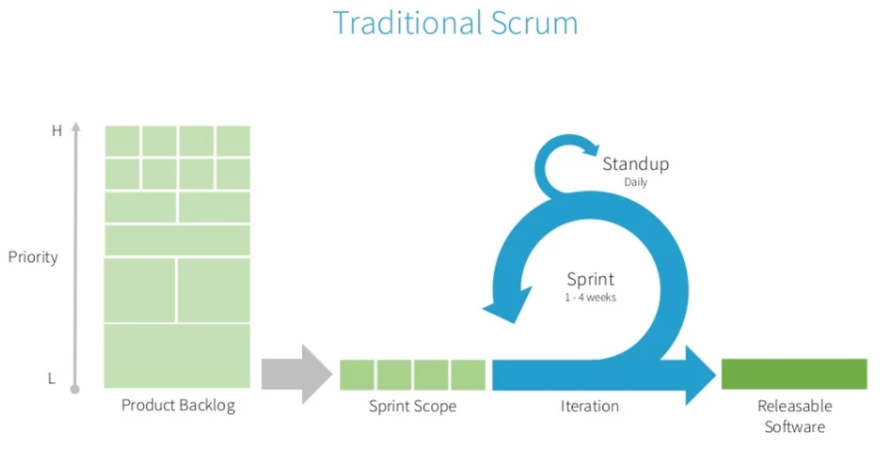
\includegraphics[width=12cm]{scrum_img.png}
\centering
\caption{Scrum framework}
\label{fig:scrum_img}
\end{figure}

Dentro de este framework trabajaremos en sprints que serán los periodos en el que se ejectuarán las tareas propuestas en la planificación. En estos sprints se espera conseguir un avance en nuestro proyecto\cite{sprint}.

\begin{figure}[h]
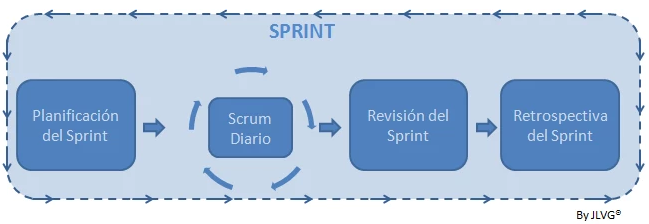
\includegraphics[width=12cm]{sprint_img.png}
\centering
\caption{Sprint de un proyecto}
\label{fig:sprint_img}
\end{figure}

\\\\
\section{Descripción del proyecto} \label{imagenes}
El planteamiento incial del juego consiste en dos mundos o escenarios, \textbf{Lanzadera Tierra-Órbita} y \textbf{Lanzadera Órtiba-Espacio}. En cada mundo se espera añadir niveles, por supuesto con distintos grados de dificultad. El primer mundo estará ligado al segundo, de forma que al completar cada nivel del primero, el usuario pueda pasar al siguiente mundo y continuar con otros niveles.

\subsection{Mundos posibles}
\subsubsection{Mundo 1: Lanzadera Tierra-Órbita} \label{EarthOrbit}
El obetivo en este escenario será alcanzar la órbita de la Tierra y posicionar allí una carga útil (un satélite, una cápsula espacial tripulada u otros dispositivos).
El usuario podrá elegir uno de los distintos cohetes que se tendrá en stock y lanzarlo al espacio, cada uno con diferentes configuraciones y con un propósito en específico. El usuario podrá controlar la dirección, la separación de etapas del cohete y el encendido del motor, además del despliegue de la carga útil que lleve al espacio. 
\\\\
Además, el usario podrá ver en tiempo real la telemetría del cohete, tales como velocidad, combustible disponible en cada etapa, inclinación del cohete, tiempo de la trayectoria, altitud, entre otros a considerar.
\\\\
Se espera interactuar también con la carga útil puesta en la órtiba de la Tierra, como la cápsula espacial, de forma que esta se maniobre para lograr una reentrada y aterrizaje.
\\\\
En la Figura (\ref{fig:trayect_surfaceOrbit}), se representa las etapas de un lanzamiento de un cohete espacial, desde la ignición, el despliegue de la carga útil en la órbita terrestre, hasta el aterrizaje de una cápsula tripulada.
\\

\begin{figure}[h]
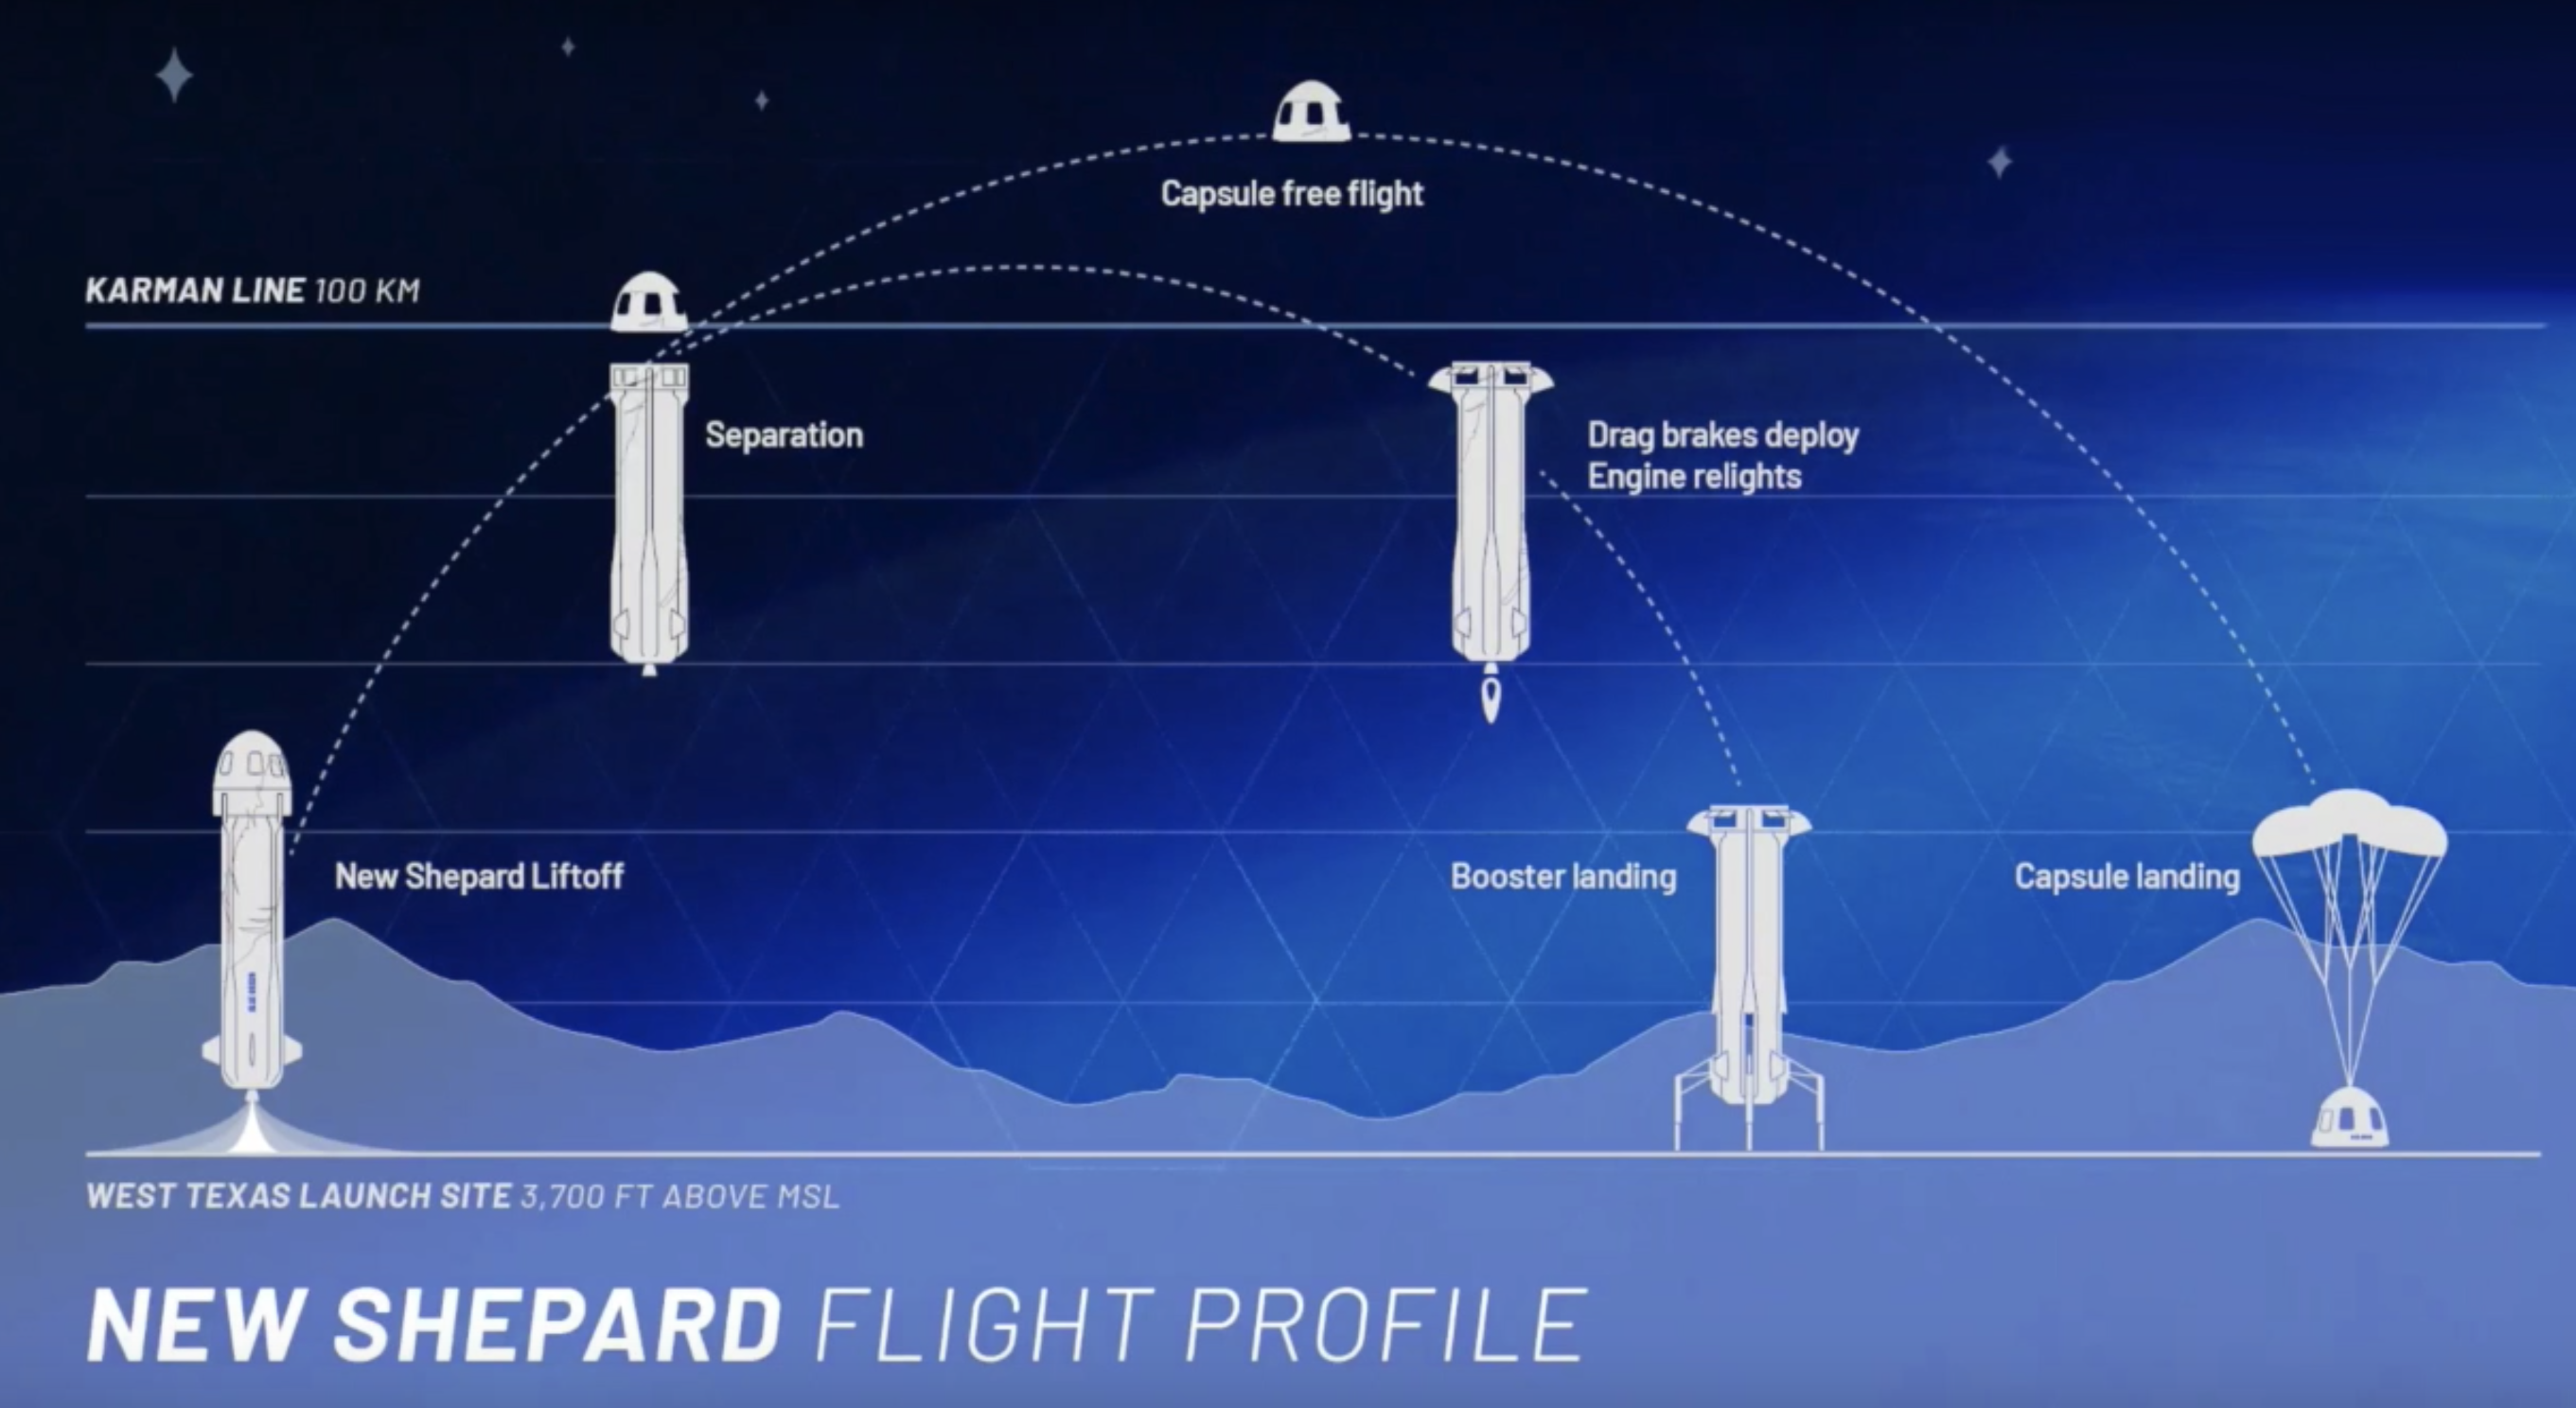
\includegraphics[width=12cm]{trayect_surfaceOrbit.png}
\centering
\caption{Etapas de lanzamiento del cohete New Shepard de Blue Origin\cite{surfaceOrbit}}
\label{fig:trayect_surfaceOrbit}
\end{figure}

\subsubsection{Mundo 2: Lanzadera Órbita-Espacio}
Una vez superado el mundo anterior de la subsección \ref{EarthOrbit}, nuestro cohete espacial estará orbitando la Tierra. El objetivo será alcanzar la órbita de otros cuerpos celestes como la Luna, los planetas del sistema solar, asteroides, entre otros a considerar. Los cuerpos celestes estarán en movimiento orbital, y el usuario apuntará en la dirección que considere que logrará acercarce al cuerpo sin chocar contra este o salirse de la trayectoria.
\\\\
Cada cuerpo celeste tendrá una configuración de gravedad distinta que afectará la trayectoria del cohete. En cada nivel se pondrán obstáculos como asteroides, planteas, lunas u otros elementos a considerar, que se interpongan entre el cohete y el cuerpo.
\\\\
En la Figura (\ref{fig:trayect_EarthMoon}), vemos que el cohete lanzado desde la órbita del planeta Tierra logra interceptar la órbita de la Luna. Este sería el objetivo que se esperaría cumplir para pasar al siguiente nivel.
\\\

\begin{figure}[h]
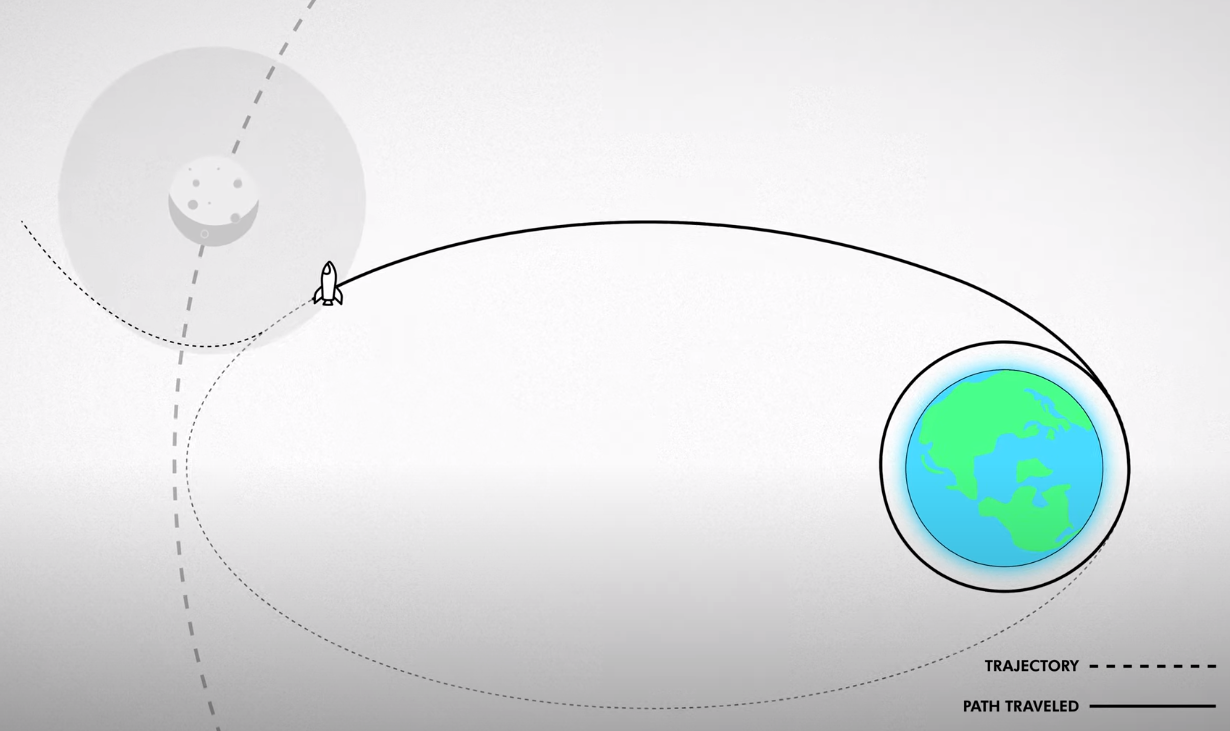
\includegraphics[width=12cm]{trayect_EarthMoon.png}
\centering
\caption{Trayectoria desde la Tierra a un cuerpo celeste\cite{earthMoon}}
\label{fig:trayect_EarthMoon}
\end{figure}

\subsection{Interfaz general de usuario}
El desarrollo de la interfaz seguramente cambiará en el transcurso del proyecto, pero podemos considerar los siguientes items como generales para un videojuego. 

\begin{itemize}
    \item Creación de usuario
    \item Tabla de records de usuarios
    \item Guardar partida
    \item Captura de pantalla
    \item Crear cohete y cuerpos celestes con parámetros específicos.
\end{itemize}

\clearpage
\bibliographystyle{IEEEtran}
\bibliography{references}

\end{document}
